\chapter[Singular values: Information]{Singular values:\\ Information}

\section{Introduction}
We have explored a very natural interpretation of the singular values are factors arbitrating the difference between the different length scales of the domain and codomain. Now we will take a very different vantage point and look at singular values as bits of information which describe details in images. This involves truncating the spectrum of singular values.

Many are familiar with the photo on the cover of Demmel's delightful book which shows low rank approximations of a photo. We will perform the same type of approximation here using an image of Camille Jordan. Besides showing the obligatory low rank approximations, we will look at the error in the approximations. Also, we will look at block structures and reversals of the domain matrices.

Besides seeing low rank approximation in action, we will look at the tradeoff between storing an entire image and storing a rank reduced SVD.

Next we alter the images through convolutions to see how this will see how this affects the spectrum of singular values.

Finally we look at structure variations. First by looking at block, then by rotating columns and rows.

\begin{figure}[h!] %  figure placement: here, top, bottom, or page
   \centering
   \includegraphics[]{pdf/"ch 06"/Jordan/"06 Jordan array"} 
   \caption[A photograph of Camille Jordan]{A photograph, in full resolution, of Camille Jordan, a pioneer of the \svdl. In matrix form, this image has $m=326$ rows and $n=266$ columns and has rank $\rho = 266$. The data are scaled to the interval $\brac{0,1}$, where 0 is black and 1 is white. What do the low rank approximations look like? \\ \ \\ There are 86,716 ( 326 $\times$ 266 ) entries in the array. An approximation of rank $\rhohat$ contains $593 \rhohat$ numbers. This implies that we must use no more than the first 146 singular values if we want to save storage space.}
   \label{fig:06:Camille}
\end{figure}

\clearpage
%%
%\input{chapters/"ch 07"/"simple objects"}
\section{A look at Camille}
Here are some plots;

\begin{figure}[htbp] %  figure placement: here, top, bottom, or page
   \centering
   \includegraphics[ ]{pdf/"ch 06"/"Camille intensity"} \\[25pt]
   \includegraphics[ ]{pdf/"ch 06"/"Camille sigma"} 
   \caption[Characterizing the image]{Characterizing the image of Camille Jordan. On the top we see the intensity distribution for every pixel. The brightest pixels have intensity 1; the darkest intensity 0. Below that we see the singular value spectrum for the 266 singular values. }
   \label{fig:CamilleCharacterization}
\end{figure}

In this section we wish to extend the standard presentation of image compression using the SVD.

Let's apply these procedures to a a photograph. The sample here is one of the father's of the SVD, Camille Jordan.

The matrix dimensions are these:
\begin{equation}
  \begin{array}{ccccc}
    \A{}          & = & \Y{} & \sig{} & \X{T} \\
    \by{326}{266} & = & \by{326}{326} & \by{326}{266} & \by{266}{266}
  \end{array}
\end{equation}

How much information is needed to store the picture as an array of reals? A total of 86,716 ( = 326 $\times$ 266 ) reals are needed.
How much information is needed to store the picture in SVD form? Here we would use the thin SVD, and

Call the total data volume $V(k)$.
\begin{table}[htdp]
\begin{center}
\begin{tabular}{lcl}
Source & dimensions & total \\
$\Y{}$ & $\by{326}{k}$ & $326k$\\
$\sig{}$ & $\by{k}{1}$ & $k$\\
$\X{}$ & $\by{266}{k}$ & $266k$\\\hline
Sum && $593k$
\end{tabular}
\end{center}
\label{tab:jordan:reals}
\caption[The census of numbers in an SVD]{The census of numbers in an SVD.}
\end{table}%

In full form, $V(266) = 593\times266 = 157,738$, an extra burden of over 80\%. The break even point is when we include the first $k=146$ singular values.

\clearpage
\break

\begin{table}[htdp]
\begin{center}
\begin{tabular}{ccc}
 & reconstituted image & error \\
 & $\hat{\A{}}$ & $\A{} - \hat{\A{}}$ \\
266 & \includegraphics[ width = 1.75in ]{pdf/fourier/Jordan_0266} & \includegraphics[ width = 1.75in ]{pdf/fourier/Jordan_diff_0266} \\
265 & \includegraphics[ width = 1.75in ]{pdf/fourier/Jordan_0265} & \includegraphics[ width = 1.75in ]{pdf/fourier/Jordan_diff_0265}\\
260 & \includegraphics[ width = 1.75in ]{pdf/fourier/Jordan_0260} & \includegraphics[ width = 1.75in ]{pdf/fourier/Jordan_diff_0260}\\
\end{tabular}
\end{center}
\label{default}
\caption[Subtract from the bottom]{Subtract from the bottom. Notice the error using almost all of the singular values. The picture contents 266 singular values.}
\end{table}%
%%%
\begin{table}[htdp]
\begin{center}
\begin{tabular}{ccc}
 & reconstituted image & error \\
 & $\hat{\A{}}$ & $\A{} - \hat{\A{}}$ \\
 15 & \includegraphics[ width = 1.75in ]{pdf/fourier/Jordan_0015} & \includegraphics[ width = 1.75in ]{pdf/fourier/Jordan_diff_0015} \\
 10 & \includegraphics[ width = 1.75in ]{pdf/fourier/Jordan_0010} & \includegraphics[ width = 1.75in ]{pdf/fourier/Jordan_diff_0010}\\
  5 & \includegraphics[ width = 1.75in ]{pdf/fourier/Jordan_0005} & \includegraphics[ width = 1.75in ]{pdf/fourier/Jordan_diff_0005}\\
\end{tabular}
\end{center}
\label{default}
\caption[Add from the top]{Add from the top. A surprisingly small number of singular values are able to convey most of the image information. Both the decomposition and the error contains a quality image also.}
\end{table}%
%%%
\begin{table}[htdp]
\begin{center}
\begin{tabular}{ccc}
 & reconstituted image & error \\
 & $\hat{\A{}}$ & $\A{} - \hat{\A{}}$ \\
  3 & \includegraphics[ width = 1.75in ]{pdf/fourier/Jordan_0003} & \includegraphics[ width = 1.75in ]{pdf/fourier/Jordan_diff_0003} \\
  2 & \includegraphics[ width = 1.75in ]{pdf/fourier/Jordan_0002} & \includegraphics[ width = 1.75in ]{pdf/fourier/Jordan_diff_0002}\\
  1 & \includegraphics[ width = 1.75in ]{pdf/fourier/Jordan_0001} & \includegraphics[ width = 1.75in ]{pdf/fourier/Jordan_diff_0001}\\
\end{tabular}
\end{center}
\label{default}
\caption[Add from the top]{Add from the top. A surprisingly small number of singular values are able to convey most of the image information. Most of the image information is in the error.}
\end{table}%

\endinput

%%%
\subsection{A look at Camille Jordan}
We really have a knack for faces.

The singular values are all set to unity
\begin{equation}
  \sig{} = \mat{c}{\I{470}\\\zero}.
\end{equation}
\begin{equation}
  \sig{-1} = \mat{cc}{\I{470}&\zero}.
\end{equation}


\begin{figure}[htbp] %  figure placement: here, top, bottom, or page
   \centering
   \includegraphics[ width = 3.71248in ]{pdf/fourier/Jordan_shadow} \\[5pt]
   $\A{} = \Y{} \mat{c}{\I{470}\\\zero} \X{T}$
   \caption{Replace the singular values spectrum with units. }
   \label{fig:fourier:Hilbert:unit}
\end{figure}

\begin{figure}[htbp] %  figure placement: here, top, bottom, or page
   \centering
   \includegraphics[  width = 5in  ]{pdf/fourier/Jordan_shadow_pi}  \\[5pt]
   $\A{T} = \X{} \mat{cc}{\I{470} & \zero} \Y{T}$
   \caption[The inverse is readily available and is the transpose]{The inverse is readily available and is the transpose. $\A{} = \X{} \Y{T}$}
   \label{fig:fourier:Hilbert:pi}
\end{figure}

\clearpage

%%%
\subsection{Convolution}
\begin{table}[htdp]
\begin{center}
\begin{tabular}{ccccc}
&
\includegraphics[ width = 1.15in ]{pdf/fourier/convolution/kernel_box} & 
\includegraphics[ width = 1.15in ]{pdf/fourier/convolution/kernel_disk} &
\includegraphics[ width = 1.15in ]{pdf/fourier/convolution/kernel_diamond} & 
\includegraphics[ width = 1.15in ]{pdf/fourier/convolution/kernel_cross} \\ [5pt] 
%%
1 &
\includegraphics[ width = 1.15in ]{pdf/fourier/convolution/box_001} & 
\includegraphics[ width = 1.15in ]{pdf/fourier/convolution/disk_001} &
\includegraphics[ width = 1.15in ]{pdf/fourier/convolution/diamond_001} & 
\includegraphics[ width = 1.15in ]{pdf/fourier/convolution/cross_001} \\ [5pt] 
%%
16 &
\includegraphics[ width = 1.15in ]{pdf/fourier/convolution/box_016} & 
\includegraphics[ width = 1.15in ]{pdf/fourier/convolution/disk_016} &
\includegraphics[ width = 1.15in ]{pdf/fourier/convolution/diamond_016} & 
\includegraphics[ width = 1.15in ]{pdf/fourier/convolution/cross_016} \\ [5pt] 
%%
31 &
\includegraphics[ width = 1.15in ]{pdf/fourier/convolution/box_031} & 
\includegraphics[ width = 1.15in ]{pdf/fourier/convolution/disk_031} & 
\includegraphics[ width = 1.15in ]{pdf/fourier/convolution/diamond_031} & 
\includegraphics[ width = 1.15in ]{pdf/fourier/convolution/cross_031} \\ [5pt]
%%
46 &
\includegraphics[ width = 1.15in ]{pdf/fourier/convolution/box_046} & 
\includegraphics[ width = 1.15in ]{pdf/fourier/convolution/disk_046} &
\includegraphics[ width = 1.15in ]{pdf/fourier/convolution/diamond_046} & 
\includegraphics[ width = 1.15in ]{pdf/fourier/convolution/cross_046} \\ [5pt] 
\end{tabular}
\end{center}
\label{default}
\caption{default}
\end{table}%

\clearpage
\begin{landscape}
\thispagestyle{empty}
\begin{table}[htdp]
\begin{center}
\begin{tabular}{cc}
\includegraphics[ width = 3.75in ]{pdf/fourier/convolution/box_sigma} & \qquad
\includegraphics[ width = 3.75in ]{pdf/fourier/convolution/disk_sigma} \\[15pt]
\includegraphics[ width = 3.75in ]{pdf/fourier/convolution/diamond_sigma} & \qquad
\includegraphics[ width = 3.75in ]{pdf/fourier/convolution/cross_sigma} \\[5pt]
\end{tabular}
\end{center}
\label{default}
\caption{Convolution operations.}
\end{table}%
\end{landscape}

%%%
\subsection{Shifting columns and rows}
\begin{equation}
  \begin{split}
    \Y{} & = \mat{c|c|c|c}{y_{1} & y_{2} & \dots & y_{n}}\\
    \Y{}_{s} & = \mat{c|c|c|c|c|c|c|c}{y_{s+1} & y_{s+2} & \dots & y_{n} & y_{1} & y_{2} & \dots & y_{s}}\\    
  \end{split}
\end{equation}
%%
\begin{equation}
  \A{} = \Y{}\,\sig{}\,\mat{c|c}{\X{}_{*,151-n} & \X{}_{*,1-150}}^{\mathrm{T}}
\end{equation}

\begin{figure}[htbp] %  figure placement: here, top, bottom, or page
   \centering
   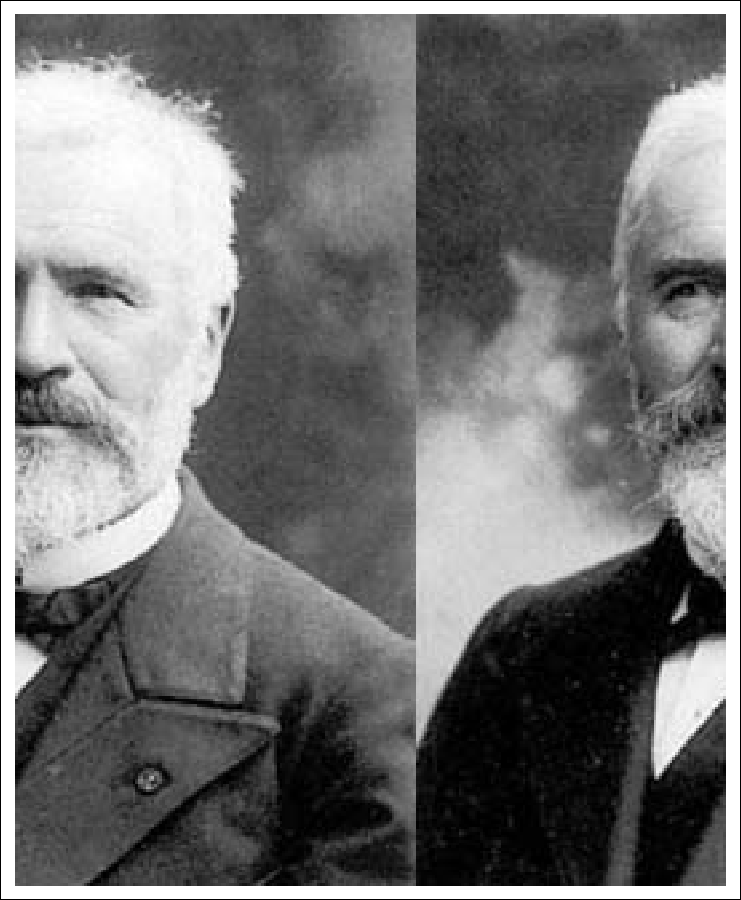
\includegraphics[ width = 2in ]{pdf/fourier/Jordan/shifts/shift_rotate_X_150} 
   \caption{}
   \label{fig:example}
\end{figure}
\clearpage

\begin{landscape}
\thispagestyle{empty}
\begin{table}[htdp]
\begin{center}
\begin{tabular}{ccc}
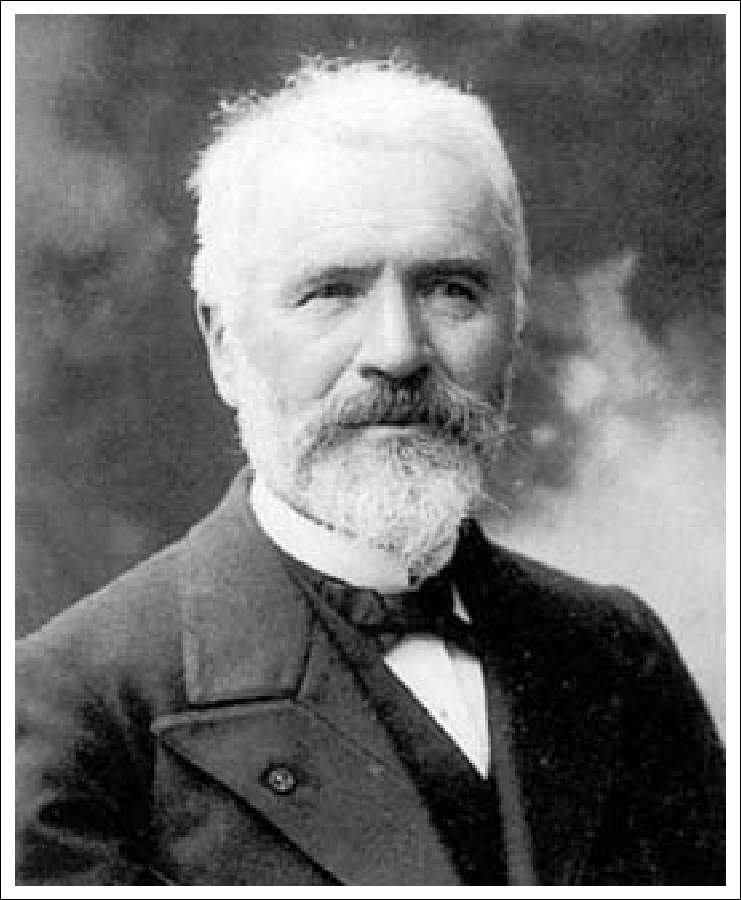
\includegraphics[ width = 2.75in ]{pdf/fourier/Jordan/shifts/shifts_good_X} &
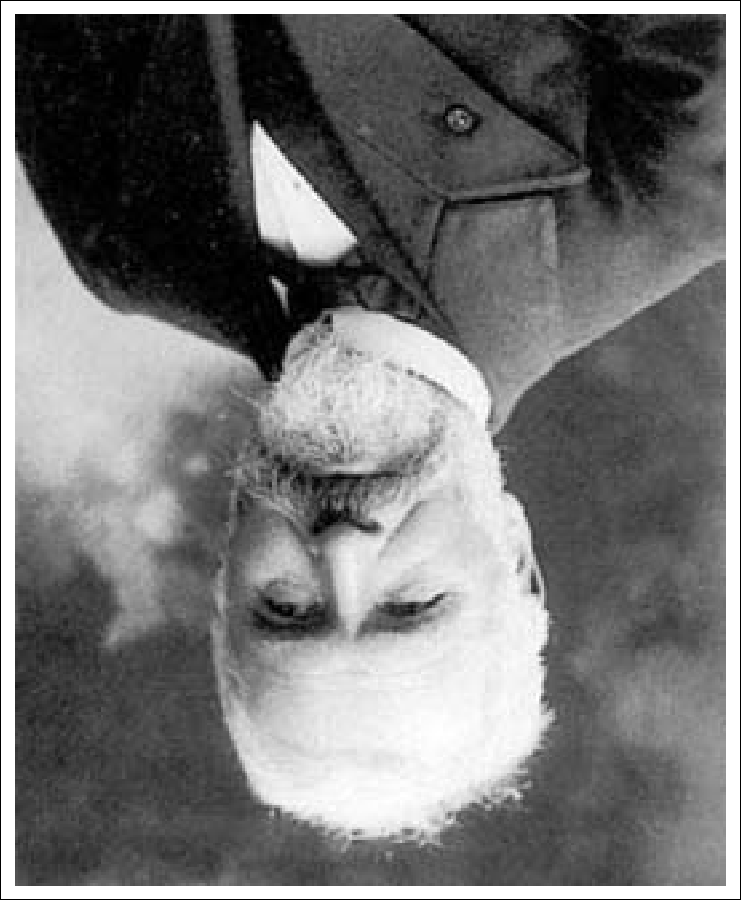
\includegraphics[ width = 2.75in ]{pdf/fourier/Jordan/shifts/shifts_good_Y} &
\includegraphics[ width = 2.75in ]{pdf/fourier/Jordan/shifts/shifts_good_X_Y} \\
$\A{}=\Y{}\,\sig{}\,\paren{\K{n}\X{}}^{\mathrm{T}}$ &
$\A{}=\paren{\K{m}\Y{}}\,\sig{}\,\X{T}$ &
$\A{}=\paren{\K{m}\Y{}}\,\sig{}\,\paren{\K{n}\X{}}^{\mathrm{T}}$ \\
$\dots$ &
$\dots$ &
$\dots$ \\
reverse rows in $\X{}$ &
reverse rows in $\Y{}$ &
reverse rows in $\X{}$ and $\Y{}$\\[5pt]
right-left flip &
up-down flip &
right-left, up-down flip\\[5pt]
\end{tabular}
\end{center}
\label{default}
\caption{Complete row shifts are valid operations.}
\end{table}%

\clearpage
\thispagestyle{empty}
\begin{table}[htdp]
\begin{center}
\begin{tabular}{ccc}
\includegraphics[ width = 2.75in ]{pdf/fourier/Jordan/shifts/shifts_bad_X} &
\includegraphics[ width = 2.75in ]{pdf/fourier/Jordan/shifts/shifts_bad_Y} &
\includegraphics[ width = 2.75in ]{pdf/fourier/Jordan/shifts/shifts_bad_X_Y} \\
$\A{}=\Y{}\,\sig{}\,\paren{\X{}\K{n}}^{\mathrm{T}}$ &
$\A{}=\paren{\Y{}\K{m}}\,\sig{}\,\X{T}$ &
$\A{}=\paren{\Y{}\K{m}}\,\sig{}\,\paren{\X{}\K{n}}^{\mathrm{T}}$ \\
$\dots$ &
$\dots$ &
$\dots$ \\
reverse columns in $\X{}$ &
reverse columns in $\Y{}$ &
reverse columns in $\X{}$ and $\Y{}$\\[5pt]
\end{tabular}
\end{center}
\label{default}
\caption{Complete column shifts are invalid operations. A few representative operations show that complete row shifts destroy the image information.}
\end{table}%

\clearpage
\thispagestyle{empty}
\begin{table}[htdp]
\begin{center}
\begin{tabular}{ccc}
\includegraphics[ width = 2.75in ]{pdf/fourier/Jordan/shifts/shift_rotate_X_150} &
\includegraphics[ width = 2.75in ]{pdf/fourier/Jordan/shifts/shift_rotate_Y_200} &
\includegraphics[ width = 2.75in ]{pdf/fourier/Jordan/shifts/shift_rotate_Y_200_X_150} \\
$\X{} \quad \to \quad \mat{c}{\X{}_{*,151-n} \\\hline \X{}_{*,1-150}}$ &
$\Y{} \to \mat{c}{\Y{}_{*,201-m} \\\hline \Y{}_{*,1-200}}$ &
$\X{} \to \mat{c}{\X{}_{*,151-n} \\\hline \X{}_{*,1-150}}$ \\ &&
$\Y{} \to \mat{c}{\Y{}_{*,201-m} \\\hline \Y{}_{*,1-200}}$ \\[10pt]
\end{tabular}
\end{center}
\label{default}
\caption{Shifting column vectors. When the column vectors of the domain matrix $\X{}$ are pushed to the right, the image moves to the right. Here the shift is 150 columns. When the column vectors of the codomain matrix $\Y{}$ are pushed to the right, the image moves up. The moves are independent as shown in the third image where both domain matrices are shifted.}
\end{table}%
\end{landscape}

%%%
\subsection{Block operations}
\clearpage
\break
\begin{equation*}
  \begin{split}
    \mathbb{A} & =
    \mat{ccccc}{ \Y{} & \Y{} & \Y{} & \Y{} & \Y{} \\ \Y{} & \Y{} & \Y{} & \Y{} & \Y{} \\ \Y{} & \Y{} & \Y{} & \Y{} & \Y{} \\ \Y{} & \Y{} & \Y{} & \Y{} & \Y{} \\ \Y{} & \Y{} & \Y{} & \Y{} & \Y{} } \,
    \mat{ccccc}{ \sig{} & \sig{} & \sig{} & \sig{} & \sig{} \\ \sig{} & \sig{} & \sig{} & \sig{} & \sig{} \\ \sig{} & \sig{} & \sig{} & \sig{} & \sig{} \\ \sig{} & \sig{} & \sig{} & \sig{} & \sig{} \\ \sig{} & \sig{} & \sig{} & \sig{} & \sig{} } \,
    \mat{ccccc}{ \X{} & \X{} & \X{} & \X{} & \X{} \\ \X{} & \X{} & \X{} & \X{} & \X{} \\ \X{} & \X{} & \X{} & \X{} & \X{} \\ \X{} & \X{} & \X{} & \X{} & \X{} \\ \X{} & \X{} & \X{} & \X{} & \X{} }^{\mathrm{T}} \\
  \end{split}
\end{equation*}

\includegraphics[ ]{pdf/"ch 07"/Jordan_5_5}

\clearpage
\break

%%
%%
\begin{equation*}
  \mathbb{A} = 
  \mat{ccccc}{ \Y{} & \zero & \zero & \zero & \zero \\ \zero & \Y{} & \zero & \zero & \zero \\ \zero & \zero & \Y{} & \zero & \zero \\ \zero & \zero & \zero & \Y{} & \zero \\ \zero & \zero & \zero & \zero & \Y{} } \,
  \mat{ccccc}{ \sig{} & \zero & \zero & \zero & \zero \\ \zero & \sig{} & \zero & \zero & \zero \\ \zero & \zero & \sig{} & \zero & \zero \\ \zero & \zero & \zero & \sig{} & \zero \\ \zero & \zero & \zero & \zero & \sig{} } \,
  \mat{ccccc}{ \X{} & \zero & \zero & \zero & \zero \\ \zero & \X{} & \zero & \zero & \zero \\ \zero & \zero &\X{} &  \zero & \zero \\ \zero & \zero & \zero & \X{} & \zero \\ \zero & \zero & \zero & \zero & \X{} }^{\mathrm{T}}
\end{equation*}

\includegraphics[ ]{pdf/"ch 07"/Jordan_I_5_5}
\clearpage


\begin{equation}
  \includegraphics[ width = 1.25in ]{pdf/"ch 07"/Jordan_I_5_5_A} = 
  \includegraphics[ width = 1.25in ]{pdf/"ch 07"/Jordan_I_5_5_Y} \, 
  \includegraphics[ width = 1.25in ]{pdf/"ch 07"/Jordan_I_5_5_S} \,
  \includegraphics[ width = 1.25in ]{pdf/"ch 07"/Jordan_I_5_5_X}
\end{equation}

\begin{equation}
  \includegraphics[ width = 1.25in ]{pdf/"ch 07"/Jordan_5_5_A} = 
  \includegraphics[ width = 1.25in ]{pdf/"ch 07"/Jordan_5_5_Y} \, 
  \includegraphics[ width = 1.25in ]{pdf/"ch 07"/Jordan_5_5_S} \,
  \includegraphics[ width = 1.25in ]{pdf/"ch 07"/Jordan_5_5_X}
\end{equation}

%%%
\subsection{Block operations 2}
\clearpage
\break
\begin{equation*}
  \begin{split}
    \mathbb{A} & =
    \mat{cc}{ \Y{} & \Y{} \\ \Y{} & \Y{}} \,
    \mat{cc}{ \sig{} & \sig{} \\ \sig{} & \sig{}} \,
    \mat{cc}{ \X{} & \X{} \\ \X{} & \X{}}^{\mathrm{T}} \\
  \end{split}
\end{equation*}

\includegraphics[ ]{pdf/"ch 07"/Jordan_2_2_A}

\clearpage
\break

%%
%%
\begin{equation}
  \mathbb{A} = 
  \mat{ccccc}{ \Y{} & \zero \\ \zero & \Y{}} \,
  \mat{ccccc}{ \sig{} & \zero \\ \zero & \sig{}} \,
  \mat{ccccc}{ \X{} & \zero \\ \zero & \X{}}^{\mathrm{T}}
\end{equation}

\includegraphics[ ]{pdf/"ch 07"/Jordan_I_2_2}
\clearpage


\begin{equation}
  \includegraphics[ width = 1.25in ]{pdf/"ch 07"/Jordan_I_2_2_A} = 
  \includegraphics[ width = 1.25in ]{pdf/"ch 07"/Jordan_I_2_2_Y} \, 
  \includegraphics[ width = 1.25in ]{pdf/"ch 07"/Jordan_I_2_2_S} \,
  \includegraphics[ width = 1.25in ]{pdf/"ch 07"/Jordan_I_2_2_X}
\end{equation}

\begin{equation}
  \includegraphics[ width = 1.25in ]{pdf/"ch 07"/Jordan_2_2_A} = 
  \includegraphics[ width = 1.25in ]{pdf/"ch 07"/Jordan_2_2_Y} \, 
  \includegraphics[ width = 1.25in ]{pdf/"ch 07"/Jordan_2_2_S} \,
  \includegraphics[ width = 1.25in ]{pdf/"ch 07"/Jordan_2_2_X}
\end{equation}


\endinput
\clearpage
\break

\section{Reordering columns and rows}
Can we use the SVD components to construct a mirror image? Can we shift the image to the left? What operations can we execute on the component matrices which still preserve an image?

This section explores how changes in the structure of the SVD components affect the image. Basically, we can only manipulate the domain matrices. There are two operations which preserve the image:
\begin{enumerate}
\item \emph{arbitrary} rotating of the \emph{columns},
\item \emph{complete} reversal of the \emph{rows}.
\end{enumerate}

%%%
\subsection{Shifting columns and rows}
For example, shifting the columns means rotating the column vectors as in this example where we rotate through the first $s$ column vectors. The original domain matrix looks like this:
\begin{equation}
  \begin{split}
    \X{} & = \mat{cccc|cccc}{x_{1} & x_{2} & \dots & x_{s} & x_{s+1} & x_{s+2} & \dots & x_{n}} .
  \end{split}
\end{equation}
The shifted domain matrix then becomes this:
\begin{equation}
  \begin{split}
    \X{}_{s} & = \mat{cccc|cccc}{x_{s+1} & x_{s+2} & \dots & x_{n} & x_{1} & x_{2} & \dots & x_{s}} .  
  \end{split}
\end{equation}
In the discussion that follows, we apply all operations (shift, reverse) to the $\X{}$ matrix before forming the transpose. Then we will see that the reconstructed image $\A{} = \Y{} \, \sig{} \, \X{T}_{s}$ has the form
\begin{equation}
  \A{}_{s} = \mat{cccc|cccc}{a_{s+1} & a_{s+2} & \dots & a_{n} & a_{1} & a_{2} & \dots & a_{s}}.
\end{equation}
Think of these shifts as the result of a shift operator, here a shifted identity matrix. Consider the example of $\I{3,1}$:
\begin{equation}
  \I{3,1} = \mat{ccc}{
  0 & 0 & 1 \\\hline
  1 & 0 & 0 \\
  0 & 1 & 1}
\end{equation}
In the example above we can now state that shifting the columns vectors $s$ spaces to the right is expressed as this:
\begin{equation}
  \X{}_{s} = \X{}\,\I{n,s}.
\end{equation}
The operation $\I{n,s}\X{}$ shifts the row vectors down $s$ spaces.

What happens when we shift $\Y{}$? What happens when we shift $\X{}$ and $\Y{}$? What happens when we shift the rows in $\X{}$ and $\Y{}$?


%%%
\subsection{Reversing column and row order}
We can also reverse the order of the rows and columns using a permutation matrix $\K{n}$. These entries $k_{rc}$ in these matrices are defined in the following manner:
\begin{equation}
  k_{rc} = 
  \begin{cases}
  1 & r + c = n + 1\\
  0 & \text{otherwise}
  \end{cases}
\end{equation}
A simple example is this:
\begin{equation}
  \K{3} = \kthree.
\end{equation}
Premultiplication by $\K{j}$ reverses the row ordering, postmultiplication reverses the column ordering. Let $\B{}\in\Accmn$. Then we would have the following:
\begin{equation}
  \begin{split}
    \K{m}\,\B{} & = \K{m} 
    \mat{c}{r_{1} \\ \vdots \\ r_{m}} = 
    \mat{c}{r_{m} \\ \vdots \\ r_{1}}, \\
    \B{}\,\K{n} & =  
    \mat{ccc}{c_{1} & \dots & c_{n}}\K{n} = 
    \mat{ccc}{c_{n} & \dots & c_{1}}.
  \end{split}
\end{equation}
Some may prefer the arrow notation:
\begin{equation}
  \begin{split}
    \K{m}\,\B{} & = \ \Updownarrow \B{}, \\
    \B{}\,\K{n} & = \ \Leftrightarrow \B{}.
  \end{split}
\end{equation}


\clearpage
\break

\begin{landscape}
\thispagestyle{empty}
\begin{table}[htdp]
\begin{center}
\begin{tabular}{ccc}
\includegraphics[ width = 2.75in ]{pdf/"ch 06"/shift/"shift col horiz"} &
\includegraphics[ width = 2.75in ]{pdf/"ch 06"/shift/"shift col vert"} &
\includegraphics[ width = 2.75in ]{pdf/"ch 06"/shift/"shift col both"} \\
$\X{} \qlraq \paren{ \X{}\,\I{n,200}}^{T}$ &
$\Y{} \qlraq \Y{}\,\I{m,100}$ &
$\X{} \qlraq \paren{ \X{}\,\I{n,200}}^{T}$ \\ &&
$\Y{} \qlraq \Y{}\,\I{m,100}$ \\
$\dots$ &
$\dots$ &
$\dots$ \\
shift $\X{}$ to left by 200 columns &
shift $\Y{}$ to left by 100 columns &
shift columns in $\X{}$ and $\Y{}$\\[5pt]
shift image left by 200 pixels &
shift image down by 100 pixels &
shift image left and down\\[5pt]
\end{tabular}
\end{center}
\label{tab:Jordan:shift}
\caption[Partial column shifts are valid operations]{Partial column shifts are valid operations. Rotating the columns shifts the image down and to the left.}
\end{table}%
\end{landscape}


\clearpage
\break

\begin{landscape}
\thispagestyle{empty}
\begin{table}[htdp]
\begin{center}
\begin{tabular}{ccc}
\includegraphics[ width = 2.75in ]{pdf/"ch 06"/shift/"flip rl"} &
\includegraphics[ width = 2.75in ]{pdf/"ch 06"/shift/"flip bt"} &
\includegraphics[ width = 2.75in ]{pdf/"ch 06"/shift/"flip both"} \\
$\X{} \qlraq \K{n}\X{}$ &
$\Y{} \qlraq \K{m}\Y{}$ &
$\X{} \qlraq \K{n}\X{}$ \\ &&
$\Y{} \qlraq \K{m}\Y{}$ \\
$\dots$ &
$\dots$ &
$\dots$ \\
reverse rows in $\X{}$ &
reverse rows in $\Y{}$ &
reverse rows in $\X{}$ and $\Y{}$\\[5pt]
right-left flip in $\A{}$ $\Longleftrightarrow$ &
up-down flip in $\A{}$ $\Updownarrow$ &
right-left, up-down flip \ $\Updownarrow \negthickspace \negthickspace  \negmedspace  \negmedspace \negmedspace  \Longleftrightarrow$\\[5pt]
\end{tabular}
\end{center}
\label{tab:Jordan:reverse}
\caption{Complete row reversals are valid operations.}
\end{table}%
\end{landscape}

\clearpage
\break

\begin{landscape}
\thispagestyle{empty}
\begin{table}[htdp]
\begin{center}
\begin{tabular}{ccc}
\includegraphics[ width = 2.75in ]{pdf/"ch 06"/shift/"shift fail a"} &
\includegraphics[ width = 2.75in ]{pdf/"ch 06"/shift/"shift fail b"} &
\includegraphics[ width = 2.75in ]{pdf/"ch 06"/shift/"shift fail both"} \\
$\Y{} \qlraq \Y{}\,\K{m}$ &
$\Y{} \qlraq \I{m,100}\Y{}$ &
$\Y{} \qlraq \K{m}\,\X{}\,\I{m,100}$\\[5pt]
\end{tabular}
\end{center}
\label{tab:Jordan:shift:fail}
\caption[Transformations which destroy the image]{Transformations which destroy the image.}
\end{table}%
\end{landscape}

%%%%
\section{Shifting singular values}
Shifting the singular values has dire consequences. A 
sv shift spectrum001

\begin{table}[htdp]
\begin{center}
\begin{tabular}{cc}
\includegraphics[ width = 1in ]{pdf/"ch 06"/shift/"sv shift 001"} &
\includegraphics[ width = 1.85in ]{pdf/"ch 06"/shift/"sv shift spectrum001"} \\
%%%
\includegraphics[ width = 1in ]{pdf/"ch 06"/shift/"sv shift 002"} &
\includegraphics[ width = 1.85in ]{pdf/"ch 06"/shift/"sv shift spectrum002"} \\
%%%
\includegraphics[ width = 1in ]{pdf/"ch 06"/shift/"sv shift 005"} &
\includegraphics[ width = 1.85in ]{pdf/"ch 06"/shift/"sv shift spectrum005"} \\
%%%
\includegraphics[ width = 1in ]{pdf/"ch 06"/shift/"sv shift 010"} &
\includegraphics[ width = 1.85in ]{pdf/"ch 06"/shift/"sv shift spectrum010"} \\
%%%
\includegraphics[ width = 1in ]{pdf/"ch 06"/shift/"sv shift 050"} &
\includegraphics[ width = 1.85in ]{pdf/"ch 06"/shift/"sv shift spectrum050"} \\
\end{tabular}
\end{center}
\label{tab:jordan:svshift}
\caption{default}
\end{table}%


\clearpage
%%%%
\subsection{Summary}
The only reo

\begin{table}[htdp]
\begin{center}
\begin{tabular}{l|cc}
 operation & preserves image & destroys image \\\hline
 reversal  & $\K{m}\X{}$    & $\X{} \, \K{m}$ \\
 shift     & $\I{m,s}\X{}$  & $\X{} \, \I{m,s}$
\end{tabular}
\end{center}
\label{tab:Jordan:shift:summary}
\caption[Image preserving operations on the domain matrices]{Image preserving operations on the rows and columns of the domain matrices.}
\end{table}%


\endinput
\subsection{Block forms}

This structure survives as expected when the blocks are embedded. The ordering of the singular values forces the domain matrices to change structure.
\begin{equation}
  \begin{split}
    \svda{T}\\
    \mat{c|c}{\mathcal{J}_{2}&\zero\\\hline \zero&\I{2}} &=\mat{cc|cc}{1&1&0&0 \\ 0&1&0&0 \\\hline 0&0&1&0 \\ 0&0&0&1} \\ 
    &=\sqrt{\frac{1}{10}}
    \mat{cccc}{\alpha_{+}&0&0&-\alpha_{-} \\ \alpha_{+}&0&0&\sqrt{20}\alpha_{+}^{-1} \\ 0&0&\sqrt{10}&0 \\ 0&\sqrt{10}&0&0}  
    \mat{cccc}{\beta_{+}&0&0&0 \\ 0&1&0&0 \\ 0&0&1&0 \\ 0&0&0&\beta_{-}}
    \sqrt{\frac{1}{10}}
    \mat{cccc}{\alpha_{-} & \alpha_{+}&0&0 \\ 0&0&0&\sqrt{10} \\ 0&0&\sqrt{10}&0 \\ -\alpha_{+}&\sqrt{20}\alpha_{+}^{-1}&0&0}
  \end{split}
\end{equation}

\endinput
\clearpage
\break

\section{Pixelation}
What happens to the singular value spectrum, as we slowly decrease the information in the image by pixelation? In this section we will start with a square image with 256 pixels to a side and reduce each dimension in half. That is, the output matrix $\tilde{\A{}}$ will have half the size of the input matrix $\A{}$:
\begin{equation}
  \A{}_{mn} \mapsto \tilde{\A{}}_{\frac{m}{2},\frac{n}{2}}.
\end{equation}
This is done by averaging four neighboring pixels to create a new pixel value like so:
\begin{equation}
  \tilde{\A{}}_{1,1} = \recip{4} \paren{ \A{}_{1,1} + \A{}_{1,2} + \A{}_{2,1} + \A{}_{2,2} }.
\end{equation}


\begin{table}[htdp]
\begin{center}
\begin{tabular}{cccc}
 image & intensity spectrum & singular value spectrum \\
\includegraphics[ width = 1.1in ] {pdf/"ch 06"/pixels/"01 Jordan pixels image"} &
\includegraphics[ width = 1.75in ]{pdf/"ch 06"/pixels/"01 Jordan pixels ints"} &
\includegraphics[ width = 1.75in ]{pdf/"ch 06"/pixels/"01 Jordan pixels sigma"} \\
%
\includegraphics[ width = 1.1in ] {pdf/"ch 06"/pixels/"02 Jordan pixels image"} &
\includegraphics[ width = 1.75in ]{pdf/"ch 06"/pixels/"02 Jordan pixels ints"} &
\includegraphics[ width = 1.75in ]{pdf/"ch 06"/pixels/"02 Jordan pixels sigma"} \\
%
\includegraphics[ width = 1.1in ] {pdf/"ch 06"/pixels/"03 Jordan pixels image"} &
\includegraphics[ width = 1.75in ]{pdf/"ch 06"/pixels/"03 Jordan pixels ints"} &
\includegraphics[ width = 1.75in ]{pdf/"ch 06"/pixels/"03 Jordan pixels sigma"} \\
%
\includegraphics[ width = 1.1in ] {pdf/"ch 06"/pixels/"04 Jordan pixels image"} &
\includegraphics[ width = 1.75in ]{pdf/"ch 06"/pixels/"04 Jordan pixels ints"} &
\includegraphics[ width = 1.75in ]{pdf/"ch 06"/pixels/"04 Jordan pixels sigma"} \\
%
\includegraphics[ width = 1.1in ] {pdf/"ch 06"/pixels/"05 Jordan pixels image"} &
\includegraphics[ width = 1.75in ]{pdf/"ch 06"/pixels/"05 Jordan pixels ints"} &
\includegraphics[ width = 1.75in ]{pdf/"ch 06"/pixels/"05 Jordan pixels sigma"} \\
%
\includegraphics[ width = 1.1in ] {pdf/"ch 06"/pixels/"06 Jordan pixels image"} &
\includegraphics[ width = 1.75in ]{pdf/"ch 06"/pixels/"06 Jordan pixels ints"} &
\includegraphics[ width = 1.75in ]{pdf/"ch 06"/pixels/"06 Jordan pixels sigma"} \\
%%%%
\end{tabular}
\end{center}
\caption[The singular value spectrum changes with pixel size]{The singular value spectrum changes with pixel size. The original picture is square with 256 pixels to a side. Each step represents a reduction in half until we get to the 8 pixel width of the final image.	}
\label{tab:Jordan:pixels}
\end{table}%


\endinput
\clearpage
\break

\section{Convolution}
The previous exercise was an example of image convolution. Let's generalize the example

\begin{table}[htdp]
\begin{center}
\begin{tabular}{ccc}
filter & convolution & singular value spectrum \\
%%%
\includegraphics[ width = 1.15in ]{pdf/"ch 06"/convolve/diamond/"filter 0010"} & 
\includegraphics[ width = 1.15in ]{pdf/"ch 06"/convolve/diamond/"image 0010"} &
\includegraphics[ width = 2.25in ]{pdf/"ch 06"/convolve/diamond/"sigma 0010"} \\ [5pt] 
%%%
\includegraphics[ width = 1.15in ]{pdf/"ch 06"/convolve/diamond/"filter 0030"} & 
\includegraphics[ width = 1.05in ]{pdf/"ch 06"/convolve/diamond/"image 0030"} &
\includegraphics[ width = 2.25in ]{pdf/"ch 06"/convolve/diamond/"sigma 0030"} \\ [5pt] 
%%%
\includegraphics[ width = 1.15in ]{pdf/"ch 06"/convolve/diamond/"filter 0050"} & 
\includegraphics[ width = 1.00in ]{pdf/"ch 06"/convolve/diamond/"image 0050"} &
\includegraphics[ width = 2.25in ]{pdf/"ch 06"/convolve/diamond/"sigma 0050"} \\ [5pt] 
%%%
\includegraphics[ width = 1.15in ]{pdf/"ch 06"/convolve/diamond/"filter 0080"} & 
\includegraphics[ width = 0.85in ]{pdf/"ch 06"/convolve/diamond/"image 0080"} &
\includegraphics[ width = 2.25in ]{pdf/"ch 06"/convolve/diamond/"sigma 0080"} \\ [5pt] 
%%%
\includegraphics[ width = 1.15in ]{pdf/"ch 06"/convolve/diamond/"filter 0100"} & 
\includegraphics[ width = 0.65in ]{pdf/"ch 06"/convolve/diamond/"image 0100"} &
\includegraphics[ width = 2.25in ]{pdf/"ch 06"/convolve/diamond/"sigma 0100"} \\ [5pt] 
%%%
\end{tabular}
\end{center}
\label{default}
\caption{Convolution operations.}
\end{table}%

\begin{table}[htdp]
\begin{center}
\begin{tabular}{ccc}
filter & convolution & singular value spectrum \\
%%%
\includegraphics[ width = 1.15in ]{pdf/"ch 06"/convolve/disk/"filter 0010"} & 
\includegraphics[ width = 1.15in ]{pdf/"ch 06"/convolve/disk/"image 0010"} &
\includegraphics[ width = 2.25in ]{pdf/"ch 06"/convolve/disk/"sigma 0010"} \\ [5pt] 
%%%
\includegraphics[ width = 1.15in ]{pdf/"ch 06"/convolve/disk/"filter 0030"} & 
\includegraphics[ width = 1.05in ]{pdf/"ch 06"/convolve/disk/"image 0030"} &
\includegraphics[ width = 2.25in ]{pdf/"ch 06"/convolve/disk/"sigma 0030"} \\ [5pt] 
%%%
\includegraphics[ width = 1.15in ]{pdf/"ch 06"/convolve/disk/"filter 0050"} & 
\includegraphics[ width = 1.00in ]{pdf/"ch 06"/convolve/disk/"image 0050"} &
\includegraphics[ width = 2.25in ]{pdf/"ch 06"/convolve/disk/"sigma 0050"} \\ [5pt] 
%%%
\includegraphics[ width = 1.15in ]{pdf/"ch 06"/convolve/disk/"filter 0080"} & 
\includegraphics[ width = 0.85in ]{pdf/"ch 06"/convolve/disk/"image 0080"} &
\includegraphics[ width = 2.25in ]{pdf/"ch 06"/convolve/disk/"sigma 0080"} \\ [5pt] 
%%%
\includegraphics[ width = 1.15in ]{pdf/"ch 06"/convolve/disk/"filter 0100"} & 
\includegraphics[ width = 0.65in ]{pdf/"ch 06"/convolve/disk/"image 0100"} &
\includegraphics[ width = 2.25in ]{pdf/"ch 06"/convolve/disk/"sigma 0100"} \\ [5pt] 
%%%
\end{tabular}
\end{center}
\label{default}
\caption{Convolution operations.}
\end{table}%

\begin{table}[htdp]
\begin{center}
\begin{tabular}{ccc}
filter & convolution & singular value spectrum \\
%%%
\includegraphics[ width = 1.15in ]{pdf/"ch 06"/convolve/cross/"filter 0010"} & 
\includegraphics[ width = 1.15in ]{pdf/"ch 06"/convolve/cross/"image 0010"} &
\includegraphics[ width = 2.25in ]{pdf/"ch 06"/convolve/cross/"sigma 0010"} \\ [5pt] 
%%%
\includegraphics[ width = 1.15in ]{pdf/"ch 06"/convolve/cross/"filter 0030"} & 
\includegraphics[ width = 1.05in ]{pdf/"ch 06"/convolve/cross/"image 0030"} &
\includegraphics[ width = 2.25in ]{pdf/"ch 06"/convolve/cross/"sigma 0030"} \\ [5pt] 
%%%
\includegraphics[ width = 1.15in ]{pdf/"ch 06"/convolve/cross/"filter 0050"} & 
\includegraphics[ width = 1.00in ]{pdf/"ch 06"/convolve/cross/"image 0050"} &
\includegraphics[ width = 2.25in ]{pdf/"ch 06"/convolve/cross/"sigma 0050"} \\ [5pt] 
%%%
\includegraphics[ width = 1.15in ]{pdf/"ch 06"/convolve/cross/"filter 0080"} & 
\includegraphics[ width = 0.85in ]{pdf/"ch 06"/convolve/cross/"image 0080"} &
\includegraphics[ width = 2.25in ]{pdf/"ch 06"/convolve/cross/"sigma 0080"} \\ [5pt] 
%%%
\includegraphics[ width = 1.15in ]{pdf/"ch 06"/convolve/cross/"filter 0100"} & 
\includegraphics[ width = 0.65in ]{pdf/"ch 06"/convolve/cross/"image 0100"} &
\includegraphics[ width = 2.25in ]{pdf/"ch 06"/convolve/cross/"sigma 0100"} \\ [5pt] 
%%%
\end{tabular}
\end{center}
\label{default}
\caption{Convolution operations.}
\end{table}%

%%%%
\subsection{How much information is in the edges?}
Filter:
\begin{equation}
  \mat{crc}{
  1 &  1 & 1 \\
  1 & -8 & 1 \\
  1 &  1 & 1 }
\end{equation}
\begin{equation}
  \begin{split}
     \sigma_{1} &= 10.2,\\
     \sigma_{n} &= 0.00461.
  \end{split}
\end{equation}
Sobol mask for vertical edges:
\begin{equation}
  \mat{rrr}{
  -1 & 0 & 1 \\
  -2 & 0 & 2 \\
  -1 & 0 & 1 }
\end{equation}
\begin{equation}
  \begin{split}
     \sigma_{1} &= 23.5,\\
     \sigma_{n} &= 0.136.
  \end{split}
\end{equation}
%%%
Sobol mask for horizontal edges:
\begin{equation}
  \mat{rrr}{
  -1 & -2 & -1 \\
   0 &  0 &  0 \\
   1 &  2 &  1 }
\end{equation}
\begin{equation}
  \begin{split}
     \sigma_{1} &= 27.4,\\
     \sigma_{n} &= 0.00000399.
  \end{split}
\end{equation}
\begin{table}[htdp]
\begin{center}
\begin{tabular}{ccc}
\includegraphics[ width = 1.6in ]{pdf/"ch 06"/convolve/edge/"edges all image"} &
\includegraphics[ width = 2.85in ]{pdf/"ch 06"/convolve/edge/"edges all spectrum"} \\
%%
\includegraphics[ width = 1.6in ]{pdf/"ch 06"/convolve/edge/"edges vert image"} &
\includegraphics[ width = 2.85in ]{pdf/"ch 06"/convolve/edge/"edges vert spectrum"} \\
%%
\includegraphics[ width = 1.6in ]{pdf/"ch 06"/convolve/edge/"edges horz image"} &
\includegraphics[ width = 2.85in ]{pdf/"ch 06"/convolve/edge/"edges horz spectrum"} \\
\end{tabular}
\end{center}
\label{tab:Jordan:edge}
\caption[Singular values and edges]{Partial column shifts are valid operations. Rotating the columns shifts the image down and to the left.}
\end{table}%


\endinput

\break
\clearpage

\section{Fade to gray}
In this section we study the effect of reducing the contrast. In particular we want to see how the singular value spectrum changes as the contrast is reduced. To do this we gradually force all the pixels to the mean value for the image, here 0.425068. 

Take matrix element with value $x$. We reduce this value to 0.425068 in $n$ steps. The change in each step is then
\begin{equation}
  \frac{0.425068 - x}{n}.
\end{equation}
During this contrast reduction the image will go from a matrix of rank $\rho = 266$ to final state with $\rho = 1$. What happens in between? How do the domain matrices change? The results are shown in tables \eqref{tab:jordan:images:melt:1} and  \eqref{tab:jordan:images:melt:2.}

\break
\clearpage

\begin{table}[htdp]
\begin{center}
\begin{tabular}{cccccc}
  $\A{}$ & $=$ & $\Y{}$ & $\sig{}$ & $\X{T}$ \\
  %%%
  \includegraphics[ width = 1.02in ]{pdf/"ch 07"/melting/"melting 010 000 B"} &&
  \includegraphics[ width = 1.25in ]{pdf/"ch 07"/melting/"melting 010 000 Y"}  &
  \includegraphics[ width = 1.02in ]{pdf/"ch 07"/melting/"melting 010 000 S"}  &
  \includegraphics[ width = 1.02in ]{pdf/"ch 07"/melting/"melting 010 000 Xt"} \\
  %%%
  \includegraphics[ width = 1.02in ]{pdf/"ch 07"/melting/"melting 010 004 B"} &&
  \includegraphics[ width = 1.25in ]{pdf/"ch 07"/melting/"melting 010 004 Y"}  &
  \includegraphics[ width = 1.02in ]{pdf/"ch 07"/melting/"melting 010 004 S"}  &
  \includegraphics[ width = 1.02in ]{pdf/"ch 07"/melting/"melting 010 004 Xt"} \\
  %%%
  \includegraphics[ width = 1.02in ]{pdf/"ch 07"/melting/"melting 010 008 B"} &&
  \includegraphics[ width = 1.25in ]{pdf/"ch 07"/melting/"melting 010 008 Y"}  &
  \includegraphics[ width = 1.02in ]{pdf/"ch 07"/melting/"melting 010 008 S"}  &
  \includegraphics[ width = 1.02in ]{pdf/"ch 07"/melting/"melting 010 008 Xt"} \\
  %%%
  \includegraphics[ width = 1.02in ]{pdf/"ch 07"/melting/"melting 010 009 B"} &&
  \includegraphics[ width = 1.25in ]{pdf/"ch 07"/melting/"melting 010 009 Y"}  &
  \includegraphics[ width = 1.02in ]{pdf/"ch 07"/melting/"melting 010 009 S"}  &
  \includegraphics[ width = 1.02in ]{pdf/"ch 07"/melting/"melting 010 009 Xt"} \\
  %%%
  \includegraphics[ width = 1.02in ]{pdf/"ch 07"/melting/"melting 010 010 B"} &&
  \includegraphics[ width = 1.25in ]{pdf/"ch 07"/melting/"melting 010 010 Y"}  &
  \includegraphics[ width = 1.02in ]{pdf/"ch 07"/melting/"melting 010 010 S"}  &
  \includegraphics[ width = 1.02in ]{pdf/"ch 07"/melting/"melting 010 010 Xt"} \\
\end{tabular}
\end{center}
\label{tab:jordan:images:melt:1}
\caption[Reducing contrast: SVD components]{Reducing contrast}
\end{table}%

\clearpage
\break

\begin{table}[htdp]
\begin{center}
\begin{tabular}{cccccc}
  & $\sigma$ \\
  %%%
  \includegraphics[ width = 0.255in ]{pdf/"ch 07"/melting/"melting 010 000 bar"}&
  \includegraphics[ width = 2.00in ]  {pdf/"ch 07"/melting/"melting 010 000 singular values"} \\
  %%%
  \includegraphics[ width = 0.255in ]{pdf/"ch 07"/melting/"melting 010 004 bar"}&
  \includegraphics[ width = 2.00in ]  {pdf/"ch 07"/melting/"melting 010 004 singular values"} \\
  %%%
  \includegraphics[ width = 0.255in ]{pdf/"ch 07"/melting/"melting 010 008 bar"}&
  \includegraphics[ width = 2.00in ]  {pdf/"ch 07"/melting/"melting 010 008 singular values"} \\
  %%%
  \includegraphics[ width = 0.255in ]{pdf/"ch 07"/melting/"melting 010 009 bar"}&
  \includegraphics[ width = 2.00in ]  {pdf/"ch 07"/melting/"melting 010 009 singular values"} \\
  %%%
  \includegraphics[ width = 0.255in ]{pdf/"ch 07"/melting/"melting 010 010 bar"}&
  \includegraphics[ width = 2.00in ]  {pdf/"ch 07"/melting/"melting 010 010 singular values"} \\
\end{tabular}
\end{center}
\label{tab:jordan:images:melt:2}
\caption[Reducing contrast: singular values]{The change in the singular values as the contrast is reduced to zero. The singular values are plotted on the right. On the left, we have a bar which shows how much of the gray scale is being used. The change in the singular value spectrum is rather minuscule as the contrast is reduced. The change from rank 266 to rank 1 is discrete.}
\end{table}%


\endinput
\clearpage
\break

\section{Images of the pseudoinverse}
We can learn a valuable lesson about the pseudoinverse from this image. While the image matrix is highly correlated, the inverse matrix is not correlated. This is shown in 
figure \eqref{fig:jordan:pseudoinverse:pairs}. This is a lesson we will see over and over. When we look at sparse matrices like tridiagonal matrices from finite difference equations we will see that the pseudoinverse is not sparse; in fact it will be very dense.

%%%%
\subsection{Left inverse}
Because the image matrix has full column rank, that is, $\rho = n$, the pseudoinverse is a left inverse
\begin{equation}
  \Ap = \AinvL
\end{equation}
and therefore
\begin{equation}
  \leftinv = \I{n}.
\end{equation}
Below, we look at the leading submatrix to get an idea of the two matrix products. Both matrices are diagonally dominant and look similar in figure \eqref{fig:jordan:pseudoinverse:lr} below.

\begin{equation}
  \begin{split}
     \paren{\leftinv}_{1:4,1:4}  &= \ifour,\\
     \paren{\rightinv}_{1:4,1:4} &= 
     \mat{rrrr}{
 0.877728 & 0.141599 & -0.0380709 & 0.00583182 \\
 \star    & 0.725206 & 0.178478   & -0.0395183 \\
 \star    & \star    & 0.716689   & 0.14253 \\
 \star    & \star    & \star      & 0.716547
     }.
  \end{split}
  \label{eq:jordan:pseudoinverse:lr}
\end{equation}

\begin{figure}[htbp] %  figure placement: here, top, bottom, or page
   \centering
   \includegraphics[ width = 2.66in ]{pdf/"ch 06"/pseudoinverse/"Jordan mplot"} \\[20pt]
   \includegraphics[ width = 3.26in ]{pdf/"ch 06"/pseudoinverse/"Jordan pseudoinverse"} 
   \caption[The original image and the pseudoinverse]{The original image and the pseudoinverse. The original image is highly correlated, the pseudoinverse is very random. However, if we look at the image pseudoinverse carefully we can see horizontal and vertical bands.}
   \label{fig:jordan:pseudoinverse:pairs}
\end{figure}


\begin{figure}[htbp] %  figure placement: here, top, bottom, or page
   \centering
   $\leftinv$ \\
   \includegraphics[ width = 2.66in ]{pdf/"ch 06"/pseudoinverse/"pseudoinverse AinvA"} \\[20pt]
   $\rightinv$ \\
   \includegraphics[ width = 3.26in ]{pdf/"ch 06"/pseudoinverse/"pseudoinverse AAinv"} 
   \caption[The matrix products $\leftinv$ and $\rightinv$]{The matrix products $\leftinv$ and $\rightinv$. Both matrices are diagonally dominant as seen in the matrix plots. Because the image matrix $\A{}$ has full column rank $\Ap = \AinvL$ and therefore $\leftinv = \I{266}$. This is seen in equations \eqref{eq:jordan:pseudoinverse:lr}. Notice that this figure does not distinguish between the identity matrix and the diagonally dominant matrix.}
   \label{fig:jordan:pseudoinverse:lr}
\end{figure}

%%%%
\subsection{Ghost image}
We have seen that the singular value spectrum embodies details of the image. Now instead of examining the spectrum, let's create one. The simplest spectrum would be make all singular values equal to one. Take the existing singular values in $\ess{}$ and replace them the identity matrix:
\begin{equation}
  \ess{} \qlraq \I{266}.
\end{equation}
The $\sig{}$ matrix then transforms as this
\begin{equation}
  \begin{split}
     \sig{} = \mat{c}{\ess{} \\\hline \zero} \qlraq  \hat{\Sigma} = \mat{c}{\I{266} \\\hline \zero}.
  \end{split}
\end{equation}
The new image is composed according to the following:
\begin{equation}
  \hat{\A{}} = \Y{} \, \hat{\Sigma} \, \X{T}.
\end{equation}
Because we are using an identity matrix for the singular values we know that
\begin{equation}
  \begin{split}
    \ess{} & = \ess{-1}, \\
    \hat{\Sigma}^{\pssymbol} &= \sig{T}
  \end{split}
\end{equation}
As a consequence, the pseudoinverse matrix is the transpose matrix: 
\begin{equation}
  \hat{\A{}}^{\psymbol} = \hat{\A{}}^{\TT}.
\end{equation}
What does a matrix with this property look like? Will it more closely resemble the image or the transpose?
You can see the result in figure \eqref{fig:jordan:pseudoinverse:ghost}.

\begin{figure}[htbp] %  figure placement: here, top, bottom, or page
   \centering
   $\hat{\A{}} = \Y{}\,\hat{\Sigma}\,\X{T}$ \\[10pt]
   \includegraphics[ width = 2.66in ]{pdf/"ch 06"/pseudoinverse/"Jordan ghost"} \\[20pt]
   $\hat{\A{}}^{\psymbol} = \hat{\A{}}^{\TT}= \X{}\,\hat{\Sigma}\,\Y{T}$ \\[10pt]
   \includegraphics[ width = 3.26in ]{pdf/"ch 06"/pseudoinverse/"Jordan ghost inv"} 
   \caption[Equality for the singular values]{Equality for the singular values. We can replace $\ess{}$, the matrix of singular values with an identity matrix to see how this alters the image.}
   \label{fig:jordan:pseudoinverse:ghost}
\end{figure}

\endinput
%\input{chapters/"ch 07"/comparison}

\endinput